\documentclass[a4paper, czech]{article}

\title{
	\begin{framed}
		\setstretch{1.5}
		{\large Audio elektronika (BPC/BKC-AUD)}\\
		Laboratorní úloha č. 8 (protokol)\\
		\textbf{CD přehrávač a D/A převodník}
	\end{framed}
	}
\author{Karolína A. Šebestová}
\date{14. 4. 2026, 11:00}

\usepackage[czech]{babel}
\usepackage{indentfirst}
\usepackage{graphicx}
\usepackage{float}
\usepackage[margin=1.5cm]{geometry}
\usepackage{booktabs}
\usepackage{amsmath}
\usepackage{multirow}
\usepackage{colortbl}
\usepackage{framed} % \begin{framed}
\usepackage{setspace} % \setstretch{}
\usepackage{siunitx}
\usepackage{xcolor}

\sisetup{locale = DE}

\begin{document}

\maketitle

\section{Měření}

\subsection{Měření modulové kmitočtové charakteristiky.}

\begin{equation}
    A_\text{U} = \textcolor{teal}{20 \cdot \log \frac{U_2}{U_1}} = 20 \cdot \log \frac{0{,}992}{1} = \underline{\underline{-0{,}070\,\text{dB}}}
\end{equation}

\begin{table}[H]
    \centering
    \catcode`\-=12
    \caption{Modulová kmitočtová charakteristika CD přehrávače ($U_{1\text{ef}} = 1\,$V).}
    \begin{tabular}{cccccccc}
        \toprule
        Stopa & $f$ {[}Hz{]} & $U_2$ {[}V{]} & $A_\text{U}$ {[}dB{]} & Stopa & $f$ {[}Hz{]} & $U_2$ {[}V{]} & $A_\text{U}$ {[}dB{]} \\
        \cmidrule(rl){1-4}
        \cmidrule(rl){5-8}
        6     & 1\,000       & 0,992      & -0,070      & 22    & 630        & 0,993      & -0,061      \\
        7     & 20         & 0,988      & -0,105      & 23    & 800        & 0,992      & -0,070      \\
        8     & 25         & 0,990      & -0,087      & 24    & 1\,000       & 0,992      & -0,070      \\
        9     & 31,5       & 0,990      & -0,087      & 25    & 1\,250       & 0,992      & -0,070      \\
        10    & 40         & 0,991      & -0,079      & 26    & 1\,600       & 0,991      & -0,079      \\
        11    & 50         & 0,991      & -0,079      & 27    & 2\,000       & 0,991      & -0,079      \\
        12    & 63         & 0,991      & -0,079      & 28    & 2\,500       & 0,990      & -0,087      \\
        13    & 80         & 0,991      & -0,079      & 29    & 3\,150       & 0,991      & -0,079      \\
        14    & 100        & 0,991      & -0,079      & 30    & 4\,000       & 0,990      & -0,087      \\
        15    & 125        & 0,991      & -0,079      & 31    & 5\,000       & 0,988      & -0,105      \\
        16    & 160        & 0,992      & -0,070      & 32    & 6\,300       & 0,988      & -0,105      \\
        17    & 200        & 0,992      & -0,070      & 33    & 8\,000       & 0,984      & -0,140      \\
        18    & 250        & 0,992      & -0,070      & 34    & 10\,000      & 0,979      & -0,184      \\
        19    & 315        & 0,992      & -0,070      & 35    & 12\,500      & 0,973      & -0,238      \\
        20    & 400        & 0,992      & -0,070      & 36    & 16\,000      & 0,958      & -0,373      \\
        21    & 500        & 0,992      & -0,070      & 37    & 20\,000      & 0,930      & -0,630      \\
    \bottomrule
    \end{tabular}
\end{table}

\begin{figure}[H]
    \centering
    
\includegraphics[width=0.7\textwidth]{grafy/graf1.pdf}
    \caption{Modulová kmitočtová charakteristika CD přehrávače.}
\end{figure}

\subsection{Kontrola fáze (polarity) obou kanálů CD přehrávače.}

\begin{figure}[H]
    \centering
    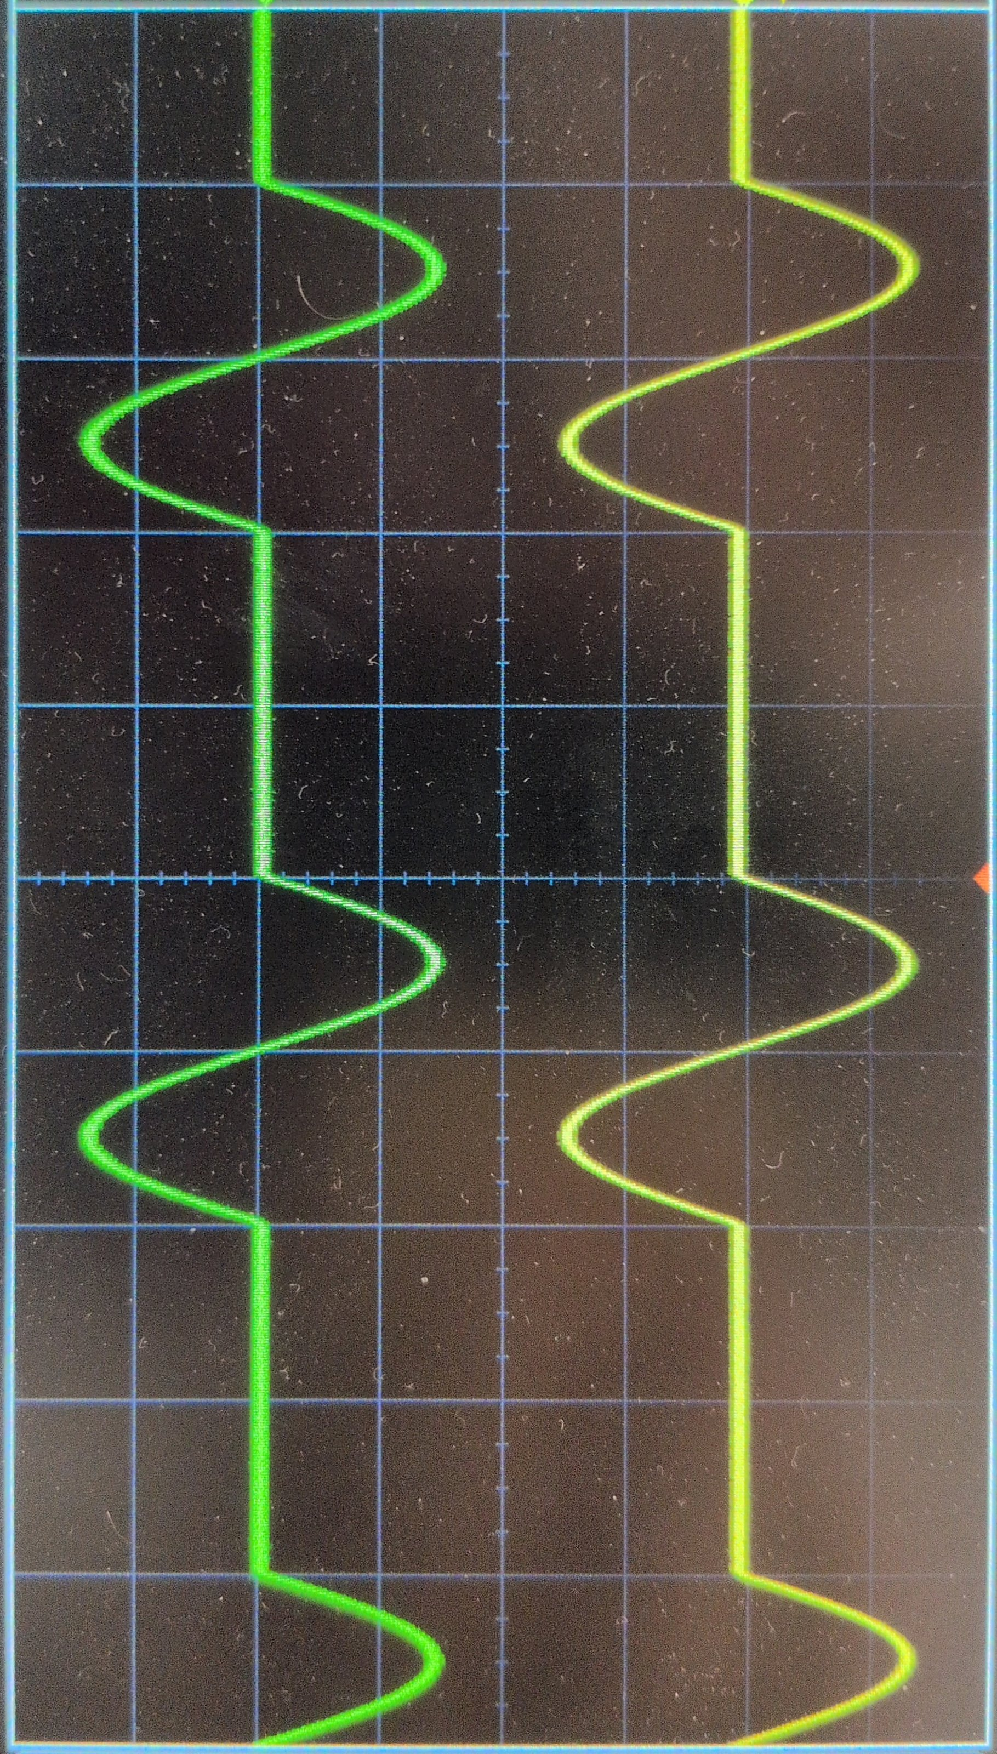
\includegraphics[height=0.7\textwidth, angle=90]{osciloskop/2_kontrola_faze.pdf}
    \caption{Průběh testovacího signálu v obou kanálech.}
\end{figure}

\subsection{Měření separace obou kanálů.}

\begin{table}[H]
    \centering
    \catcode`\-=12
    \caption{Separace kanálů ($_1 = 2\,$V).}
    \begin{tabular}{cccc}
        \toprule
        Stopa & f {[}Hz{]} & UR {[}dB{]} & UL {[}dB{]} \\
        \cmidrule(rl){1-4}
        29    & 100          & 0           & -68,05      \\
        30    & 1\,000       & 0           & -67,99      \\
        31    & 10\,000      & 0           & -67,69      \\
        32    & 20\,000      & 0           & -66,66      \\
        \bottomrule
    \end{tabular}
\end{table}

\subsection{Kontrola linearity D/A převodníku přehrávače.}

\begin{table}[H]
    \centering
    \catcode`\-=12
    \caption{Linearita D/A převodníku CD přehrávače ($f = 1\,$kHz).}
    \begin{tabular}{cccc}
        \toprule
        Stopa & $U_1$ {[}dB{]} & $U_{2\text{L}}$ {[}dB{]} & $U_{2\text{R}}$ {[}dB{]} \\
        \cmidrule(rl){1-4}
        14    & 0           & 0            & 0,08         \\
        15    & -1          & -1           & -0,92        \\
        16    & -3          & -3           & -2,92        \\
        17    & -6          & -6           & -5,92        \\
        18    & -10         & -10          & -9,92        \\
        19    & -20         & -20          & -19,92       \\
        20    & -60         & -58,83       & -58,68       \\
        21    & -80         & -67,97       & -67,66       \\
        22    & -90         & -68,32       & -67,92       \\
        \bottomrule
    \end{tabular}
\end{table}

\begin{figure}[H]
    \centering
    
\includegraphics[width=0.7\textwidth]{grafy/graf2.pdf}
    \caption{Linearita D/A převodníku CD přehrávače ($f=1\,$kHz).}
\end{figure}

\subsection{Měření odstupu signálu od šumu S/N.}

$$N = 800\,\mathrm{\mu V}$$

$$S = 2,075\,\mathrm{V}$$

\begin{equation}
    S/N = \frac{S}{N} = \frac{2,075}{800 \cdot 10^{-6}} = \underline{\underline{2593,75}}\ \text{(absolutní hodnota)}
\end{equation}

\begin{equation}
    S/N = 20 \cdot \log \frac{S}{N} = 20 \cdot \log \frac{2,075}{800 \cdot 10^{-6}} = \underline{\underline{66,28\,\text{dB}}}\ \text{(v logaritmické míře)}
\end{equation}

\subsection{Měření harmonického zkreslení THD v závislosti na úrovni signál.}

\begin{table}[H]
    \centering
    \catcode`\-=12
    \caption{Závislost harmonického zkreslení $THD = f(U_1)$ ($f = 1\,$kHz).}
    \begin{tabular}{ccc}
        \toprule
        Stopa & $U_1$ {[}dB{]} & THD {[}\%{]} \\
        \cmidrule(rl){1-3}
        14    & 0           & 0,0022       \\
        15    & -1          & 0,0024       \\
        16    & -3          & 0,003        \\
        17    & -6          & 0,0039       \\
        18    & -10         & 0,0067       \\
        19    & -20         & 0,0196       \\
        20    & -58,83      & -            \\
        21    & -67,97      & -            \\
        22    & -68,32      & -            \\
        \bottomrule
    \end{tabular}
\end{table}

\begin{figure}[H]
    \centering
    
\includegraphics[width=0.7\textwidth]{grafy/graf3.pdf}
    \caption{Závislost harmonického zkreslení na vstupním napětí.}
\end{figure}

\section{Použité měřící přístroje}

\begin{itemize}
    \item \textbf{GEN} CD generátor - disky AVP \& Marutech a Sony Test CD type 3
    \item \textbf{APA} audio analyzátor Audio Precision Portable One
    \item \textbf{OSC} digitální osciloskop Tektronix TDS 2014
    \item \textbf{CDR} měřený CD rekordér Philips CDR 796
    \item propojovací vodiče 2x CINCH - BNC, 2 x rozbočovací „T člen", 4 x XLR - CINCH
\end{itemize}

\section{Závěr}

Naměřená modulová kmitočtová charakteristika je velmi vyrovnaná, v celém měřeném pásmu 20\,Hz až 20\,kHz se přenos pohybuje v rozmezí $-0{,}061$ až $-0{,}630$\,dB.
K výraznějšímu poklesu dochází až na nejvyšších kmitočtech, maximální útlum $-0{,}630$\,dB byl naměřen při 20\,kHz.
Mezní kmitočty při poklesu o $-3$\,dB nebylo možné odečíst.

Výsledek kontroly fáze kanálů přehrávače můžeme pozorovat na obrázku 2.
Potvrdilo se, že oba kanály mají shodnou polaritu. Na osciloskopu byly pozorovány vzájemně shodné sinusové průběhy s vynechanou každou sudou periodou.

V úloze 3 jsme měřili separaci kanálů přehrávače (tabulka 2).
Naměřené hodnoty se pohybují v rozmezí $-66{,}66$ až $-68{,}05$\,dB.
Lze pozorovat, že s rostoucím kmitočtem se separace mírně zhoršuje (od $-68{,}05$\,dB při 100\,Hz po $-66{,}66$\,dB při 20\,kHz).

Výsledek kontroly linearity D/A převodníku lze pozorovat na obrázku 3.
Převodní charakteristika má lineární charakter v rozsahu $U_1 = 0$ až $-20$\,dB, kde se naměřené hodnoty obou kanálů velmi dobře shodují se vstupní úrovní.
Při nižších úrovních ($-60$ až $-90$\,dB) dochází k odchylkám od linearity, například pro $U_1 = -90$\,dB bylo naměřeno pouze $-68{,}32$\,dB (L) a $-67{,}92$\,dB (R).
Toto může být způsobeno nelinearitou převodníku nebo nepřesností měření velmi malých hodnot napětí.
Kanály přehrávače se od sebe liší minimálně.

Dále jsme měřili odstup signálu od šumu (S/N) přehrávače.
Odstup signálu od šumu nám v absolutní hodnotě vyšel $S/N = 2593{,}75$, respektive $68{,}28$\,dB v~logaritmické míře.
Šum by tedy neměl výrazně proniknout do užitečného signálu.

V poslední úloze jsme měřili závislost harmonického zkreslení THD na úrovni signálu (obrázek 4).
Naměřené hodnoty harmonického zkreslení se pohybují v tisícinách až setinách procenta, od 0,0022\,\% při plné úrovni ($U_1 = 0$\,dB) po 0,0196\,\% při $U_1 = -20$\,dB, naměřené zkreslení je tedy velmi malé.
Pro slabší signál než $-20$\,dB zkreslení nebylo možné změřit, protože signál již nebylo možné dostatečně odlišit od šumu.

\end{document}